\documentclass[10pt,aspectratio=169]{beamer}
\usepackage{uh}

\title{Annual PhD Review \#1}
\subtitle{Year 2023}
\author{Rabimba Karanjai}


\begin{document}
\sloppy

\maketitle

\section[fragile]{About Me}
\begin{frame}
\begin{columns}
\begin{column}{0.7\textwidth}
Joined the PhD Program in 2020 Fall. Was allowed to come to UH physically and resume degree in Fall 2021.
\begin{block}{Prior Work:}
\begin{enumerate}
\item \href{https://patents.google.com/patent/US11025643B2/en?q=(rabimba)&oq=rabimba}{Mobile multi-party digitally signed documents and techniques for using these allowing detection of tamper} - {2021} - {US Patent US11025643B2}
\item \href{https://scholarship.rice.edu/handle/1911/105623}{Optimizing Web Virtual Reality} - {MS Thesis}
\end{enumerate}
\end{block}
\begin{block}{Courses Taken at UH}
\begin{itemize}
\item Operating System
\item Computer Architecture
\item Machine Learning
\item Cloud Computing
\item Intro Automata \& Computability
%\item Info.Tech Management \& Control
\item Prgrm Analys \& Testing
\end{itemize}
\end{block}

\end{column}
\begin{column}{0.3\textwidth}
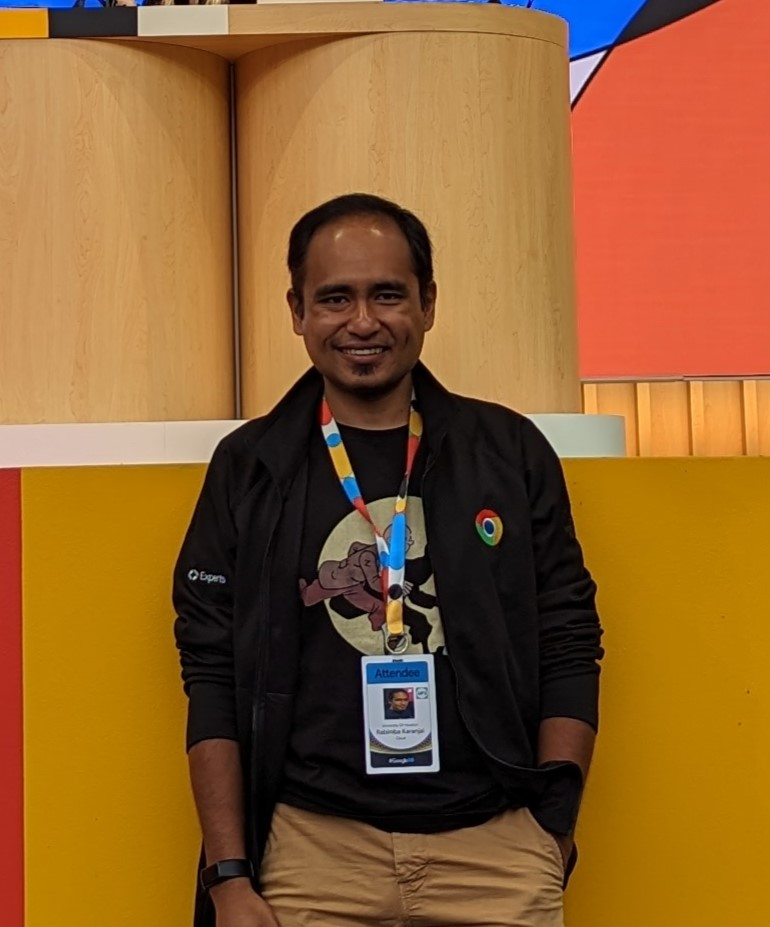
\includegraphics[width=\textwidth]{source/me}\\
\end{column}
\end{columns}
\end{frame}



\section{Collected Short Stories on Confidential Decentralized Transaction, real word use cases}

\begin{frame}{Confidential Decentralized Transaction}{\thesection \, \secname}

Today we are going to re-visit some existing problems in Decentralized Transaction systems. Different ways we explored to mitigate them, and extending them to cover real world use cases.

\begin{itemize}
\item {\href{https://dl.acm.org/doi/abs/10.1145/3465480.3466924}{\underline{An event driven framework for smart contract execution}}}  {\newline{
Mudabbir Kaleem,Keshav Kasichainula,\textbf{Rabimba Karanjai},Lei Xu,Zhimin Gao,Lin Chen,Weidong Shi}} -- {ACM DEBS} -- {2021}
\item {\href{https://ieeexplore.ieee.org/abstract/document/9461133}{\underline{On Conditional Cryptocurrency With Privacy}}} 
    {\newline{\textbf{Rabimba Karanjai}; Lei Xu; Zhimin Gao; Lin Chen; Mudabbir Kaleem; Weidong Shi}} 
    {IEEE ICBC} 
    {2021}
\item {\href{https://dl.acm.org/doi/abs/10.1145/3464298.3493401}{\underline{Privacy preserving event based transaction system in a decentralized environment}}} 
    {\newline{\textbf{Rabimba Karanjai},Lei Xu,Zhimin Gao,Lin Chen,Mudabbir Kaleem,Weidong Shi}} 
    {ACM Middleware}
    {2021}
\end{itemize}
\end{frame}

\begin{frame}{Overview of Problems}

\textbf {An event driven framework for smart contract execution} - {ACM DEBS} -- {2021}

\begin{itemize} 
\item The current smart contract platforms use a transaction-driven execution model, which requires users to initiate transactions to trigger smart contract execution. This model is inefficient, costly, and unsuitable for many time-sensitive applications that depend on external events. 
\item The existing solutions for event-driven smart contract execution rely on centralized oracles or trusted third parties to provide event triggers, which introduce security and reliability risks. Moreover, these solutions do not separate event processing from transaction processing, which limits the scalability and performance of smart contracts. 
\item The current smart contract platforms do not provide a generic and flexible framework for event-driven smart contract execution that can support various types of events, such as time-based, data-based, or user-defined events. 
\end{itemize}
\end{frame}

\begin{frame}{Overview of Problems}

\textbf {On Conditional Cryptocurrency With Privacy} - {IEEE ICBC} -- {2021}
\begin{itemize} 
\item The current cryptocurrency systems do not support conditional transactions, which are transactions that depend on the outcomes of certain events, such as sports betting, prediction markets, or insurance claims. Conditional transactions can enable new applications and use cases for cryptocurrencies, such as decentralized finance, peer-to-peer gambling, or smart insurance. 
\item The existing approaches for conditional transactions rely on smart contracts to lock and release cryptocurrencies based on event triggers, which introduce several drawbacks, such as locking assets, requiring triggering mechanisms, increasing transaction costs, and exposing event conditions to the public. 
\item The current cryptocurrency systems do not provide privacy protection for conditional transactions, which can leak sensitive information about the users’ preferences, beliefs, or risks. Privacy protection can enhance the security and usability of conditional transactions, as well as prevent manipulation or censorship by malicious actors. 
\end{itemize}
\end{frame}

\begin{frame}{Overview of Problems}
\textbf {Privacy preserving event based transaction system in a decentralized environment} - {ACM Middleware} - {2021}
\begin{itemize} 
\item The current transaction systems do not support event-based transactions, which are transactions that depend on the outcomes of certain events, such as sports betting, prediction markets, or insurance claims. Event-based transactions can enable new applications and use cases for data sharing and management, such as decentralized finance, peer-to-peer gambling, or smart insurance. 
\item The existing approaches for event-based transactions rely on smart contracts to lock and release digital assets based on event triggers, which introduce several drawbacks, such as locking assets, requiring triggering mechanisms, increasing transaction costs, and exposing event conditions to the public. 
\item The current transaction systems do not provide privacy protection for event-based transactions, which can leak sensitive information about the users’ preferences, beliefs, or risks. Privacy protection can enhance the security and usability of event-based transactions, as well as prevent manipulation or censorship by malicious actors. 
\end{itemize}
\end{frame}

\begin{frame}{Overview of Solutions}

\textbf {An event driven framework for smart contract execution} - {ACM DEBS} -- {2021}
\begin{itemize} \item The paper proposes a new design and implementation of a smart contract platform based on the event-driven execution model. The paper argues that this model is more suitable for many emerging smart contract applications that require timely execution based on events, such as decentralized finance, prediction markets, or insurance claims. \item The paper presents EDSC’s design under the Ethereum framework, and shows how it can be easily adapted for other existing smart contract platforms. The paper also demonstrates the implementation and evaluation of EDSC using Ethereum client and reports an average 2.2 to 4.6 times reduced total latency of event triggered smart contracts. \item The paper shows that the proposed system can improve the performance and scalability of smart contracts by using an event-driven execution model that separates event processing from transaction processing. The system also provides a generic and flexible framework for event-driven smart contract execution that can support various types of events, such as time-based, data-based, or user-defined events. \end{itemize}
\end{frame}

\begin{frame}{Overview of Solutions}
\textbf {On Conditional Cryptocurrency With Privacy} - {IEEE ICBC} -- {2021}
\begin{itemize} \item The paper proposes a new design and implementation of a conditional cryptocurrency system with privacy protection. The system allows users to create and transfer confidential conditional coins that are linked to the outcomes of certain events, such as sports betting, prediction markets, or insurance claims. \item The paper demonstrates how to extend the Zerocoin data model and protocol to support confidential conditional coins, and evaluates the system using xJsnark. \item The paper shows that the proposed system can enable free trade of conditional assets and prevent assets from being locked, without relying on any triggering mechanism or exposing event conditions to the public. The system also ensures that the conditional coins are secure, scalable, and compatible with existing cryptocurrency platforms. \end{itemize}
\end{frame}

\begin{frame}{Overview of Solutions}
\textbf {Privacy preserving event based transaction system in a decentralized environment} - {ACM Middleware} - {2021}
\begin{itemize} \item The paper presents the design and implementation of a privacy preserving event based UTXO (Unspent Transaction Output) transaction system. The system allows users to create and transfer confidential event based UTXO notes that are linked to the outcomes of certain events, such as sports betting, prediction markets, or insurance claims. \item The paper demonstrates how to extend the Zerocoin data model and protocols to support confidential event based UTXO notes, and evaluates the system using xJsnark. \item The paper shows that the proposed system can enable privacy preserving data sharing and management using event based UTXO notes, without relying on any triggering mechanism or exposing event conditions to the public. The system also ensures that the associations between UTXO notes and events are hidden from the validators. \end{itemize}
\end{frame}

\begin{frame}{Problems and Solutions}
\begin{itemize}
\item EDSC: An Event-Driven Smart Contract Platform
  \begin{itemize}
    \item Problem: Scalability and performance challenges of current smart contract platforms that use the transaction-driven execution model.
    \item Solution: An event-driven execution model that is more suitable for many emerging smart contract applications that require timely execution based on events.
  \end{itemize}
\item On Conditional Cryptocurrency With Privacy
  \begin{itemize}
    \item Problem: Lack of privacy in existing conditional cryptocurrency systems.
    \item Solution: A system that encodes the event outcome as part of a cryptocurrency note in a UTXO based system, and ensures that the event conditions and the coin values are hidden from public view using zero-knowledge proofs.
  \end{itemize}
\item Privacy preserving event based transaction system in a decentralized environment
  \begin{itemize}
    \item Problem: Lack of privacy in existing event based transaction systems.
    \item Solution: A system that encodes the event outcome as part of the UTXO note and protects the event privacy by hiding it with zero-knowledge proof based protocols.
  \end{itemize}
\end{itemize}
\end{frame}

\section{Securing Real World Applications}

\begin{frame}[fragile]{Decentralized Application Infrastructures}

{\href{https://ieeexplore.ieee.org/document/9805493}{\underline{Decentralized Application Infrastructures as Smart Contract Codes - \newline{\textit{Distinguished Paper}}}}}
    {\newline{\textbf{Rabimba Karanjai},Keshav Kasichainula,Nour Diallo,Mudabbir Kaleem,Lei Xu,Lin Chen,Weidong Shi}} - {IEEE ICBC} - {2022}
\begin{itemize} \item The paper proposes a new design and implementation of a smart contract platform that supports decentralized application infrastructures. The paper shows how to extend the TOSCA domain-specific language to model and specify decentralized application infrastructures as smart contract codes. \item The paper demonstrates how to deploy and manage decentralized application infrastructures using smart contract codes on the Ethereum framework, and shows how the design can be easily adapted for other existing smart contract platforms. The paper also evaluates the system using Ethereum client and reports the performance and cost metrics of the system. \item The paper shows that the proposed system can enable full decentralization in general-purpose computing using blockchain technology.  \end{itemize}
\end{frame}

\begin{frame}[fragile]{Blockchain Applications of TEE}

{\href{https://dl.acm.org/doi/abs/10.1145/3505253.3505259}{\underline{Lessons Learned from Blockchain Applications of TEE and Implications}}} 

{\textbf{Rabimba Karanjai}, L Xu, L Chen, F Zhang, Z Gao, W Shi} - {ACM HASP} - {2021}
\begin{itemize} \item The paper reviews and analyzes the existing blockchain-based applications that use hardware TEEs for various purposes, such as data privacy, off-chain computation, or consensus enhancement. The paper identifies the common patterns, challenges, and pitfalls of these applications. \item The paper discusses the implications and recommendations for future research on hardware TEEs for blockchain-based applications. The paper suggests some open problems and opportunities for improving the design and implementation of hardware TEEs in general. \item The paper provides a comprehensive survey and taxonomy of the state-of-the-art hardware TEEs and blockchain-based applications that use them. The paper also compares and contrasts the features and limitations of different hardware TEEs and blockchain-based applications. \end{itemize}
\end{frame}

\section{Can hardware help?}

\begin{frame}[fragile]{Utilizing secure Trusted Execution Environment}

\href{https://camps.aptaracorp.com/ACM_PMS/PMS/ACM/BSCI23/14/7b4e9185-e3b1-11ed-b37c-16bb50361d1f/OUT/bsci23-14.html}{\underline{Decentralized Translator of Trust:}} \underline{Supporting Heterogeneous TEE for Critical Infrastructure Protection}

{\textbf{Rabimba Karanjai}, Rowan Collier, Zhimin Gao, Lin Chen, Xinxin Fan, Taeweon Suh, Weidong Shi and Lei Xu} - {ACM BSCI} - {2023}

\begin{itemize}
\item Challenges
  \begin{itemize}
    \item Heterogeneous TEE systems are difficult to interoperate with each other.
    \item Existing solutions to this problem are either not scalable or not secure.
  \end{itemize}
\item Contributions
  \begin{itemize}
    \item We propose DHTee, a decentralized coordination mechanism that uses blockchain technology to support the interoperability of devices with different TEE.
    \item DHTee offers a unified framework to support heterogeneous TEE systems.
    \item DHTee reduces the system management complexity and can be easily extended to support new TEE schemes.
%    \item DHTee eliminates the single point of failure in the attestation process.
    \item DHTee protects information stored on the blockchain without affecting the function to support heterogeneous TEEs.
  \end{itemize}
\end{itemize}

\end{frame}

\section{Exploration}

\begin{frame}[fragile]{Privacy, LLM, Serverless, Decentralization}

 \begin{itemize}
\item Can we support emerging Web3 DAPPS in decentralized multi cloud environment? 
("Decentralized FaaS over Multi-Clouds" - Submitted to IEEE Cloud)
\item Can a system be designed that exposes serverless functions with integrity guarantees using Trusted Execution Environment?
\item Can we build a system where LLM's can be used not only to generate code, but also systematic mathematical proofs accompanying them for verification, without prohibitive overhead
\item Can we systematically test and evaluate High Performance Computing codes generated by different LLM's by generating automated test cases (To be submitted to ASPLOS)
\item Can we study the pitfalls, problems and bugs introduced when used for generating smart contracts (Will be submitted to BRAIN 2023)
\item Can we make a automated Verilog based exploit generator and code verifier for circuits?
\end{itemize}
\end{frame}


\section{Summary}

\begin{frame}
\frametitle{Conclusion}
\begin{itemize}
\item  My research direction in future will pivot more towrads providing security guarantees in code.
\item The privacy aspects of those work should mesh up well enough with decentralization aspects of the previous works.
\item Exploration of security hardwares as tools for the above two points will also be my point of interest.
\end{itemize}
\end{frame}

%\backmatter

\end{document}
